\documentclass[border=8pt]{standalone}
\usepackage[T1]{fontenc}\usepackage{lmodern}\usepackage{xspace}
\usepackage{amsmath,amssymb,amsfonts,mathtools}
\usepackage[table]{xcolor}\usepackage{graphicx}
\usepackage{tikz}\usetikzlibrary{arrows.meta,calc,fit,positioning,shapes,decorations.pathreplacing}
\setlength{\textwidth}{17cm}
% ── Colors used in the figures and tables ────────────────────────────────────
\definecolor{actcol}{HTML}{D32F2F}   % red: always active / restricted
\definecolor{arbcol}{HTML}{00A000}   % green: varying
\definecolor{parcol}{HTML}{0000FF}   % blue: parity
\colorlet{hilite}{black!12}          % one gray for everything the paper highlights

% ── Bit-index macros ─────────────────────────────────────────────────────────
% red italic = always active, green upright = varying, blue = parity,
% red box = punctured, plain black = no class.
\newcommand{\actbit}[1]{\textcolor{actcol}{\textit{#1}}}
\newcommand{\arbbit}[1]{\textcolor{arbcol}{#1}}
\newcommand{\parbit}[1]{\textcolor{parcol}{#1}}
% Robust, because it is used inside \caption, which is a moving argument.
\DeclareRobustCommand{\puncbit}[1]{\mbox{\tikz[baseline=(pb.base)]{%
  \node[draw=actcol, dashed, line width=0.5pt, rounded corners=1pt,
        inner xsep=1.6pt, inner ysep=1pt] (pb) {\ensuremath{#1}};}}}
\newcommand{\extbit}[1]{#1}                 % a bit entering a subround
\newcommand{\freebit}[1]{\parbit{#1}}       % a bit of the parity
\newcommand{\Pp}[1]{\actbit{#1}}
\newcommand{\Vv}[1]{\arbbit{#1}}

\newcommand{\CS}{2.6}
\newcommand{\PS}{11.9}
\newcommand{\RS}{17}   % row separation for the 2x2 subround panel figure
\tikzset{
  wire/.style  = {-{Latex[length=1.9mm,width=1.5mm]}, thick},
  % fig:forro-sr17-20 is two panels wide and fig:forro-sr17-22 three, so the
  % three-panel one is resized harder; the sizes below are the two-panel
  % defaults, and fig:forro-sr17-22 restates them larger to cancel that.
  rot/.style   = {draw, line width=0.7pt, rounded corners=1.2pt,
                  inner xsep=3pt, inner ysep=2.2pt,
                  font=\fontsize{13.1}{15}\selectfont},
  wname/.style = {font=\fontsize{10.9}{13}\selectfont},
  diff/.style  = {font=\fontsize{10.9}{13}\selectfont, align=center,
                  anchor=north, inner sep=1.5pt},
  title/.style = {font=\fontsize{9.1}{11}\selectfont\bfseries},
  % a word whose correlation-1 extension stops here: dashed red box + its f_i tag
  stopbox/.style = {draw=actcol, dashed, line width=0.5pt, rounded corners=1pt,
                    inner sep=2pt}
}
\newcommand{\srfops}{%
  % --- operators
  \node[opadd]  (dadd1) at ({3*\CS},-0.5) {};
  \node[opxor]  (cxor)  at ({2*\CS},-1.5) {};
  \node[opadd]  (badd)  at ({1*\CS},-2.5) {};
  \node[rot] (brot)  at ({1*\CS},-3.75) {$\lll 10$};
  \node[opadd]  (aadd1) at (0,-4.5) {};
  \node[opxor]  (exor)  at ({4*\CS},-5.2) {};
  \node[opadd]  (dadd2) at ({3*\CS},-6.0) {};
  \node[rot] (drot)  at ({3*\CS},-7.25) {$\lll 27$};
  \node[opadd]  (cadd)  at ({2*\CS},-8.0) {};
  \node[opxor]  (bxor)  at ({1*\CS},-9.0) {};
  \node[opadd]  (aadd2) at (0,-9.7) {};
  \node[rot] (arot)  at (0,-10.8)       {$\lll 8$};
  % --- vertical wires
  \draw[wire] (0,0.5) -- (aadd1);        \draw[wire] (aadd1) -- (aadd2);
  \draw[wire] (aadd2) -- (arot);         \draw[wire] (arot) -- (0,-11.7);
  \draw[wire] ({1*\CS},0.5) -- (badd);   \draw[wire] (badd) -- (brot);
  \draw[wire] (brot) -- (bxor);          \draw[wire] (bxor) -- ({1*\CS},-11.7);
  \draw[wire] ({2*\CS},0.5) -- (cxor);   \draw[wire] (cxor) -- (cadd);
  \draw[wire] (cadd) -- ({2*\CS},-11.7);
  \draw[wire] ({3*\CS},0.5) -- (dadd1);  \draw[wire] (dadd1) -- (dadd2);
  \draw[wire] (dadd2) -- (drot);         \draw[wire] (drot) -- ({3*\CS},-11.7);
  \draw[wire] ({4*\CS},0.5) -- (exor);   \draw[wire] (exor) -- ({4*\CS},-11.7);
  % --- horizontal taps (source wire -> operator)
  \draw[wire] ({4*\CS},-0.5)  -- (dadd1);   % d += e
  \draw[wire] ({3*\CS},-1.5)  -- (cxor);    % c ^= d
  \draw[wire] ({2*\CS},-2.5)  -- (badd);    % b += c
  \draw[wire] ({1*\CS},-4.5)  -- (aadd1);   % a += b
  \draw[wire] (0,-5.2)        -- (exor);    % e ^= a
  \draw[wire] ({4*\CS},-6.0)  -- (dadd2);   % d += e
  \draw[wire] ({3*\CS},-8.0)  -- (cadd);    % c += d
  \draw[wire] ({2*\CS},-9.0)  -- (bxor);    % b ^= c
  \draw[wire] ({1*\CS},-9.7) -- (aadd2);   % a += b
}
% top / bottom word names: #1..#5 = a,b,c,d,e
\newcommand{\srfin}[5]{%
  \node[wname] at (0,2) {$#1$};        \node[wname] at ({1*\CS},2) {$#2$};
  \node[wname] at ({2*\CS},2) {$#3$};  \node[wname] at ({3*\CS},2) {$#4$};
  \node[wname] at ({4*\CS},2) {$#5$};}
\newcommand{\srfout}[5]{%
  \node[wname] at (0,-12.15) {$#1$};       \node[wname] at ({1*\CS},-12.15) {$#2$};
  \node[wname] at ({2*\CS},-12.15) {$#3$}; \node[wname] at ({3*\CS},-12.15) {$#4$};
  \node[wname] at ({4*\CS},-12.15) {$#5$};}
% Mask carried in / out with correlation 1; $[\,]$ = nothing on that word.
% Nodes are named ia..ie / oa..oe so that \stopbit can box one of them.
\newcommand{\srfdiffin}[5]{%
  \node[diff] (ia) at (0,1.6) {#1};       \node[diff] (ib) at ({1*\CS},1.6) {#2};
  \node[diff] (ic) at ({2*\CS},1.6) {#3}; \node[diff] (id) at ({3*\CS},1.6) {#4};
  \node[diff] (ie) at ({4*\CS},1.6) {#5};}
\newcommand{\srfdiffout}[5]{%
  \node[diff] (oa) at (0,-12.5) {#1};       \node[diff] (ob) at ({1*\CS},-12.5) {#2};
  \node[diff] (oc) at ({2*\CS},-12.5) {#3}; \node[diff] (od) at ({3*\CS},-12.5) {#4};
  \node[diff] (oe) at ({4*\CS},-12.5) {#5};}
% \stopbit{node}{tag}: put the red puncturing box round the bit whose
% correlation-1 extension stops here, and tag it with the function it is
% punctured into, e.g. \stopbit{id}{f_1}
\newcommand{\stopbit}[2]{%
  \node[stopbox, fit=(#1)] {};
  \node[font=\scriptsize, text=actcol, anchor=north] at ($(#1.south)+(0,-0.12)$) {$#2$};}

% ── CPNB figure palette ──────────────────────────────────────────────────────
% Four fills whose lightness is well separated, so the classification survives
% black and white printing: white 100%, cpnbcol 80%, synccol 49%, restcol 26%.
% restcol is actcol darkened, so a restricted bit reads as the same red as an
% always-active bit while keeping the lightness gap these figures rely on.
\definecolor{cpnbcol}{RGB}{204,204,204}
\definecolor{synccol}{RGB}{90,125,205}
\colorlet{restcol}{actcol!70!black}

% ── Uniform figure frame ─────────────────────────────────────────────────────
% Every figure is resized to the same stated width and gets the same padding,
% whatever scale factor that figure uses. The rule is set to zero width: the
% figures are not boxed, and a visible frame would compete with the dashed red
% box, which is the one frame in this paper that carries a meaning.
% #1 is the total width of the framed result, rule and padding included.
\newlength{\figframewidth}
\newcommand{\figframe}[2]{%
  \begingroup
  \setlength{\fboxrule}{0pt}%
  \setlength{\fboxsep}{12pt}%
  \setlength{\figframewidth}{#1}%
  \addtolength{\figframewidth}{-2\fboxsep}%
  \addtolength{\figframewidth}{-2\fboxrule}%
  \fbox{\resizebox{\figframewidth}{!}{#2}}%
  \endgroup}

% ── ARX operators ────────────────────────────────────────────────────────────
% The shape carries the meaning, so the figures read correctly without colour:
% square for addition modulo $2^{32}$, circle for XOR, rounded box for
% rotation.
% Operator geometry. Defaults suit the two-panel figures; a figure that is
% resized harder or softer resets these so the printed size stays the same.
\newlength{\opsize}\setlength{\opsize}{6mm}
\newlength{\oprule}\setlength{\oprule}{0.7pt}
\tikzset{
  % modular addition: a cross across a square, i.e. $\boxplus$
  opadd/.style = {draw, line width=\oprule, rectangle, minimum size=\opsize,
                  inner sep=0pt,
                  path picture={%
                    \draw[line width=\oprule]
                      (path picture bounding box.west) --
                      (path picture bounding box.east)
                      (path picture bounding box.south) --
                      (path picture bounding box.north);}},
  % rotation: a rounded box, so that it reads as an operator alongside the
  % square addition and the round XOR without being mistaken for either
  oprot/.style = {draw, line width=\oprule, rounded corners=1.2pt,
                  minimum height=\opsize, inner xsep=3pt, inner ysep=2.2pt,
                  font=\Large},
  % XOR: a cross running the full diameter of a circle, i.e. $\oplus$
  opxor/.style = {draw, line width=\oprule, circle, minimum size=\opsize,
                  inner sep=0pt,
                  path picture={%
                    \draw[line width=\oprule]
                      (path picture bounding box.west) --
                      (path picture bounding box.east)
                      (path picture bounding box.south) --
                      (path picture bounding box.north);}}
}

% ── Differential-linear arrow ────────────────────────────────────────────────
% One spelling for every distinguisher in the paper: \dlarrow{4} etc.
\newcommand{\dlarrow}[1]{%
  \underset{\text{#1 rounds}}{\overset{\mathcal{DL}}{\longrightarrow}}}

% ── Cipher name ─────────────────────────────────────────────────────────────
\newcommand{\Forro}{Forr\'o\xspace}


\begin{document}
\begin{minipage}{0.98\textwidth}\centering

\figframe{0.98\textwidth}{%
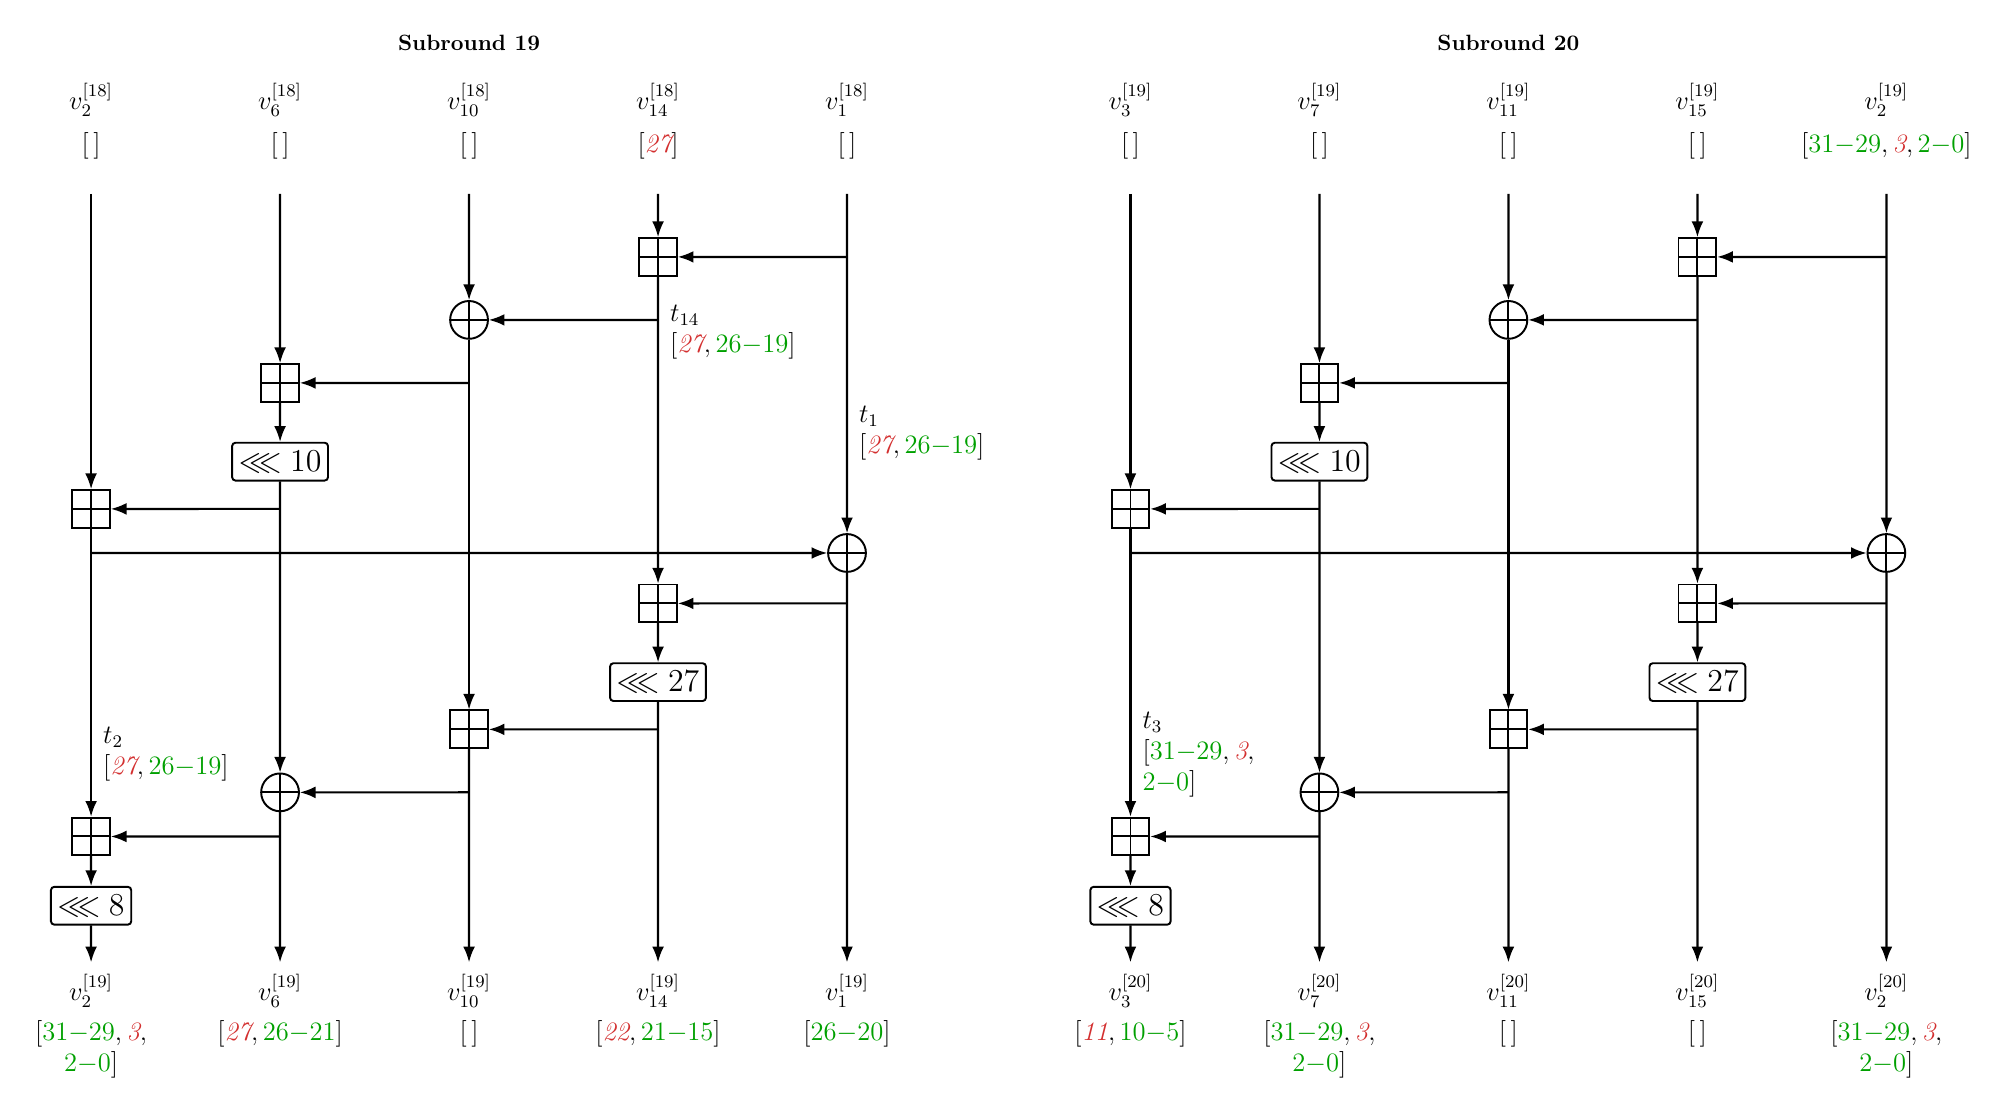
\begin{tikzpicture}[
    scale=0.8,
    every node/.style={transform shape},
    line/.style={thick},
    arrow/.style={-{Latex[length=2mm]}, thick},
    font=\large
]

\begin{scope}[xshift=0cm, yshift=0cm]
    \def\xa{0}
    \def\xb{3}
    \def\xc{6}
    \def\xd{9}
    \def\xe{12}

    \node[font=\normalsize\bfseries] at (6, 2.9) {Subround 19};

    \node at (\xa,2) {$v_{2}^{[18]}$};
    \node at (\xa,-12.15) {$v_{2}^{[19]}$};
    \node at (\xb,2) {$v_{6}^{[18]}$};
    \node at (\xb,-12.15) {$v_{6}^{[19]}$};
    \node at (\xc,2) {$v_{10}^{[18]}$};
    \node at (\xc,-12.15) {$v_{10}^{[19]}$};
    \node at (\xd,2) {$v_{14}^{[18]}$};
    \node at (\xd,-12.15) {$v_{14}^{[19]}$};
    \node at (\xe,2) {$v_{1}^{[18]}$};
    \node at (\xe,-12.15) {$v_{1}^{[19]}$};

    \node[opadd] (dadd1) at (\xd,-0.5) {};
    \node[opxor] (cxor) at (\xc,-1.5) {};
    \node[opadd] (badd) at (\xb,-2.5) {};
    \node[oprot] (brot) at (\xb,-3.75) {$\lll 10$};
    \node[opadd] (aadd1) at (\xa,-4.5) {};
    \node[opxor] (exor) at (\xe,-5.2) {};
    \node[opadd] (dadd2) at (\xd,-6) {};
    \node[oprot] (drot) at (\xd,-7.25) {$\lll 27$};
    \node[opadd] (cadd) at (\xc,-8) {};
    \node[opxor] (bxor) at (\xb,-9) {};
    \node[opadd] (aadd2) at (\xa,-9.7) {};
    \node[oprot] (arot) at (\xa,-10.8) {$\lll 8$};

    \draw[arrow] (\xa,0.5) to (aadd1);
    \draw[arrow] (aadd1) to (aadd2);
    \draw[arrow] (aadd2) to (arot);
    \draw[arrow] (arot) to (\xa,-11.7);
    \draw[arrow] (\xb,0.5) to (badd);
    \draw[arrow] (badd) to (brot);
    \draw[arrow] (brot) to (bxor);
    \draw[arrow] (bxor) to (\xb,-11.7);
    \draw[arrow] (\xc,0.5) to (cxor);
    \draw[arrow] (cxor) to (cadd);
    \draw[arrow] (cadd) to (\xc,-11.7);
    \draw[arrow] (\xd,0.5) to (dadd1);
    \draw[arrow] (dadd1) to (dadd2);
    \draw[arrow] (dadd2) to (drot);
    \draw[arrow] (drot) to (\xd,-11.7);
    \draw[arrow] (\xe,0.5) to (exor);
    \draw[arrow] (exor) to (\xe,-11.7);

    \draw[arrow] (\xe,-0.5) to (dadd1);
    \draw[arrow] (\xd,-1.5) to (cxor);
    \draw[arrow] (\xc,-2.5) to (badd);
    \draw[arrow] (\xb,-4.5) to (aadd1);
    \draw[arrow] (\xa,-5.2) to (exor);
    \draw[arrow] (\xe,-6) to (dadd2);
    \draw[arrow] (\xd,-8) to (cadd);
    \draw[arrow] (\xc,-9) to (bxor);
    \draw[arrow] (\xb,-9.7) to (aadd2);

    \node[align=center, anchor=north] at (\xa,1.6) {$[\,]$};
    \node[align=left, anchor=west, inner sep=1pt] at (\xa+0.15,-8.4) {$t_{2}$ \\ $[\actbit{27},\arbbit{26{-}19}]$};
    \node[align=center, anchor=north] at (\xa,-12.5) {$[\arbbit{31{-}29},\actbit{3},$ \\ $\arbbit{2{-}0}]$};
    \node[align=center, anchor=north] at (\xb,1.6) {$[\,]$};
    \node[align=center, anchor=north] at (\xb,-12.5) {$[\actbit{27},\arbbit{26{-}21}]$};
    \node[align=center, anchor=north] at (\xc,1.6) {$[\,]$};
    \node[align=center, anchor=north] at (\xc,-12.5) {$[\,]$};
    \node[align=center, anchor=north] at (\xd,1.6) {$[\actbit{27}]$};
    \node[align=left, anchor=west, inner sep=1pt] at (\xd+0.15,-1.7) {$t_{14}$ \\ $[\actbit{27},\arbbit{26{-}19}]$};
    \node[align=center, anchor=north] at (\xd,-12.5) {$[\actbit{22},\arbbit{21{-}15}]$};
    \node[align=center, anchor=north] at (\xe,1.6) {$[\,]$};
    \node[align=left, anchor=west, inner sep=1pt] at (\xe+0.15,-3.3) {$t_{1}$ \\ $[\actbit{27},\arbbit{26{-}19}]$};
    \node[align=center, anchor=north] at (\xe,-12.5) {$[\arbbit{26{-}20}]$};
\end{scope}

\begin{scope}[xshift=16.5cm, yshift=0cm]
    \def\xa{0}
    \def\xb{3}
    \def\xc{6}
    \def\xd{9}
    \def\xe{12}

    \node[font=\normalsize\bfseries] at (6, 2.9) {Subround 20};

    \node at (\xa,2) {$v_{3}^{[19]}$};
    \node at (\xa,-12.15) {$v_{3}^{[20]}$};
    \node at (\xb,2) {$v_{7}^{[19]}$};
    \node at (\xb,-12.15) {$v_{7}^{[20]}$};
    \node at (\xc,2) {$v_{11}^{[19]}$};
    \node at (\xc,-12.15) {$v_{11}^{[20]}$};
    \node at (\xd,2) {$v_{15}^{[19]}$};
    \node at (\xd,-12.15) {$v_{15}^{[20]}$};
    \node at (\xe,2) {$v_{2}^{[19]}$};
    \node at (\xe,-12.15) {$v_{2}^{[20]}$};

    \node[opadd] (dadd1) at (\xd,-0.5) {};
    \node[opxor] (cxor) at (\xc,-1.5) {};
    \node[opadd] (badd) at (\xb,-2.5) {};
    \node[oprot] (brot) at (\xb,-3.75) {$\lll 10$};
    \node[opadd] (aadd1) at (\xa,-4.5) {};
    \node[opxor] (exor) at (\xe,-5.2) {};
    \node[opadd] (dadd2) at (\xd,-6) {};
    \node[oprot] (drot) at (\xd,-7.25) {$\lll 27$};
    \node[opadd] (cadd) at (\xc,-8) {};
    \node[opxor] (bxor) at (\xb,-9) {};
    \node[opadd] (aadd2) at (\xa,-9.7) {};
    \node[oprot] (arot) at (\xa,-10.8) {$\lll 8$};

    \draw[arrow] (\xa,0.5) to (aadd1);
    \draw[arrow] (aadd1) to (aadd2);
    \draw[arrow] (aadd2) to (arot);
    \draw[arrow] (arot) to (\xa,-11.7);
    \draw[arrow] (\xb,0.5) to (badd);
    \draw[arrow] (badd) to (brot);
    \draw[arrow] (brot) to (bxor);
    \draw[arrow] (bxor) to (\xb,-11.7);
    \draw[arrow] (\xc,0.5) to (cxor);
    \draw[arrow] (cxor) to (cadd);
    \draw[arrow] (cadd) to (\xc,-11.7);
    \draw[arrow] (\xd,0.5) to (dadd1);
    \draw[arrow] (dadd1) to (dadd2);
    \draw[arrow] (dadd2) to (drot);
    \draw[arrow] (drot) to (\xd,-11.7);
    \draw[arrow] (\xe,0.5) to (exor);
    \draw[arrow] (exor) to (\xe,-11.7);

    \draw[arrow] (\xe,-0.5) to (dadd1);
    \draw[arrow] (\xd,-1.5) to (cxor);
    \draw[arrow] (\xc,-2.5) to (badd);
    \draw[arrow] (\xb,-4.5) to (aadd1);
    \draw[arrow] (\xa,-5.2) to (exor);
    \draw[arrow] (\xe,-6) to (dadd2);
    \draw[arrow] (\xd,-8) to (cadd);
    \draw[arrow] (\xc,-9) to (bxor);
    \draw[arrow] (\xb,-9.7) to (aadd2);

    \node[align=center, anchor=north] at (\xa,1.6) {$[\,]$};
    \node[align=left, anchor=west, inner sep=1pt] at (\xa+0.15,-8.4) {$t_{3}$ \\ $[\arbbit{31{-}29},\actbit{3},$ \\ $\arbbit{2{-}0}]$};
    \node[align=center, anchor=north] at (\xa,-12.5) {$[\actbit{11},\arbbit{10{-}5}]$};
    \node[align=center, anchor=north] at (\xb,1.6) {$[\,]$};
    \node[align=center, anchor=north] at (\xb,-12.5) {$[\arbbit{31{-}29},\actbit{3},$ \\ $\arbbit{2{-}0}]$};
    \node[align=center, anchor=north] at (\xc,1.6) {$[\,]$};
    \node[align=center, anchor=north] at (\xc,-12.5) {$[\,]$};
    \node[align=center, anchor=north] at (\xd,1.6) {$[\,]$};
    \node[align=center, anchor=north] at (\xd,-12.5) {$[\,]$};
    \node[align=center, anchor=north] at (\xe,1.6) {$[\arbbit{31{-}29},\actbit{3},\arbbit{2{-}0}]$};
    \node[align=center, anchor=north] at (\xe,-12.5) {$[\arbbit{31{-}29},\actbit{3},$ \\ $\arbbit{2{-}0}]$};
\end{scope}

\end{tikzpicture}}

\par\medskip
\begin{minipage}{\linewidth}\small\setlength{\parindent}{0pt}
\textbf{Trail of $f_1$ in the $5$-round attack, subrounds 19 and 20.} Each panel is one subround of \Forro: its five words enter at the top and leave at the bottom, and the boxes are the modular additions, XORs and rotations of the subround. The bracket under a word lists the active bits of its mask. \actbit{Red italic} bits are active in every kept trail, \arbbit{green} bits are active only in some of them, and $[\,]$ means that the word carries no active bit. A label $t_j$ gives the mask of the intermediate value on branch $j$ at the marked point. The enumeration starts from the target bit $v^{[18]}_{14}[27]$ at the top of subround 19 and follows the trails through the two subrounds. The masks at the bottom of subround 20 are on the last state $V^{[20]}$; the final key addition $\bar z_j = v^{[20]}_j \boxplus k_j$ then turns them into masks on keystream bits and key bits.
\end{minipage}
\end{minipage}
\end{document}
